%# -*- coding: utf-8-unix -*-
%%==================================================
%% chapter02.tex for SJTU Master Thesis
%% Encoding: UTF-8
%%==================================================

%1,展开差分隐私定义,laplace,讨论维度问题
%2,展开面向决策树的差分隐私设计,典型方案


\chapter{相关背景技术}
\label{chap:background}

\section{引言}

上一章描述了课题所涉及的背景知识及相关问题的研究现状,本章将介绍理论知识及问题模型。主要内容为差分隐私相关的数学定义和重要概念介绍,以及频率矩阵加噪模型描述。

\section{差分隐私}

\subsection{差分隐私定义}

%给定数据集$D$,另一数据集$D'$和它至多相差一条记录。
在差分隐私中,我们希望某个在数据集上的运算结果不因任意一条记录的改变而变化明显。也就是说,某个算法在改变前后的两个数据集上做运算,其输出上的差别不至于披露任意一条特定数据项。

\begin{defn}
	
($\varepsilon$\textsc{-差分隐私})\cite{Dwork Calibrating} 数据集$D$和$D'$至多相差一条记录,即$|D$$\triangle$$D'|$ $\leqslant$ 1。一个随机算法$\partial$满足$\varepsilon$-差分隐私,当且仅当对于$\partial$任意可能的输出$O$,我们有下式成立:

\begin{equation}
  \label{eq:res1}
	 Pr[\partial(D) = O] \leqslant e^{\varepsilon} \cdot Pr[\partial(D') = O]
\end{equation}


其中,$Pr$表示事件发生的概率,在此也表示隐私被披露的风险。$\varepsilon$为隐私预算,$\varepsilon$越小,算法的隐私保护程度越高。

\end{defn}

实现差分隐私的主要方法是对真实值添加噪音扰动,而噪音量的量级大小是由全局敏感性(Sensitivity)来定义。它表示数据集发生改变时,某一函数运算在输出结果上产生的最大距离。

\begin{defn}
	(\textsc{全局敏感性}\cite{Dwork Calibrating}) 数据集$D$和$D'$至多相差一条记录,即$|D$$\triangle$$D'|$ $\leqslant$ 1。函数$\mathcal{F}$的查询维度为d,并且有$\mathcal{F}$:$D \rightarrow \mathrm{R}^d$。那么,函数$\mathcal{F}$的全局敏感性$S(\mathcal{F})$定义为:
\begin{equation}
\label{eq:res2}
	S(\mathcal{F}) = \max \limits_{D,D'} \| \mathcal{F}(D) - \mathcal{F}(D') \|_{1}
\end{equation}

其中,$\|\cdot\|$表示$L_{1}$范数。
\end{defn}



\subsection{差分隐私实现机制}

基于全局敏感性,本课题涉及两种加噪算法:拉普拉斯机制(Laplace mechanism)和指数机制(Exponential mechanism)。

\begin{thm}
	\label{thm:res1}
	(\textsc{拉普拉斯机制}\cite{Dwork Calibrating}) 在数据集$D$中,有函数$\mathcal{F}$: $D\rightarrow \mathrm{R}^d$,若算法$\mathcal{M}$满足下式,则$\mathcal{M}$满足$\varepsilon$-差分隐私:
	\begin{equation}
	\mathcal{M}(D) = \mathcal{F}(D) + (\textit{Laplace}(S(\mathcal{F})/ \varepsilon)^d
	\end{equation}
	其中,\textit{Laplace}为标准的拉普拉斯分布,$S(\mathcal{F})/\varepsilon$决定噪音量级。
\end{thm}
例如,当$\mathcal{F}$为计数函数时,S($\mathcal{F}$)=1,此时$\mathcal{M}(D) = \mathcal{F}(D) + (\textit{Laplace}(1/\varepsilon)^d$。

指数机制通过设计打分函数对属性进行打分计算,分值越高就有越大的概率被选中。
\begin{thm}
	\label{thm:res2}
	(\textsc{指数机制}\cite{exponential}) 有数据集$D$,打分函数$\mathcal{F}$: ($D$ $\times$ $O$)$\rightarrow$ $\mathrm{R}$,对每个输出项o$\in$ $O$都对应一个打分值。对于若算法$\mathcal{M}$满足下式,则$\mathcal{M}$满足$\varepsilon$-差分隐私:
	\begin{equation}
	\mathcal{M}(D,\mathcal{F}) = \{o \in O: Pr(o)\wasypropto exp(\frac{\varepsilon\mathcal{F}(D,o)}{2S(\mathcal{F})}) \}
	\end{equation}
	其中,S($\mathcal{F}$)为打分函数$\mathcal{F}$的全局敏感性,Pr(o)表示返回输出项o的概率。
\end{thm}
在决策树分类算法中,常用的打分有信息增益,基尼指数等。通过算法$\mathcal{M}$得到候选属性的概率值分布,之后按照概率抽取属性。

\section{频率矩阵及问题表述}

频率矩阵是个基本的统计模型,基于频率矩阵实现的差分隐私算法满足了基本的隐私保护需求,但是在范围计数查询应用中存在着缺陷——随着查询维度的增加,累加的噪音值不断逼近真实值,严重影响性能扩展性---这也是本课题要着力解决的问题。

\subsection{频率矩阵模型}

引用\ref{sec:weidu}节中介绍立方表(Cuboid)的假设背景,此时选取原表的全部属性构建立方表,即Cuboid{性别,年龄,成绩},也就是原表的频率矩阵。如图\ref{fig:frequency}(a)为原表,\ref{fig:frequency}(b)为对应的频率矩阵。

\begin{figure}[!htp]
	\centering
	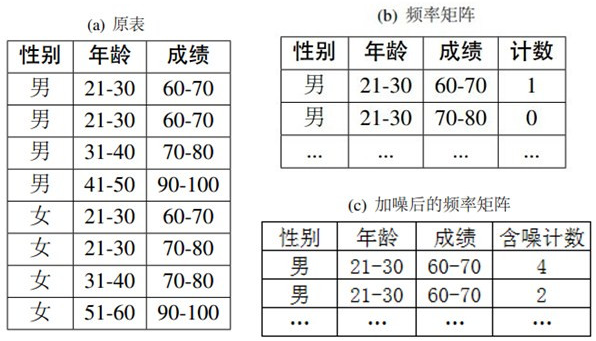
\includegraphics[width=5in]{chap2/frequency}
	\bicaption[fig:frequency]{图}{频率矩阵示例}{Fig.}{Sample frequency matrix}
\end{figure}

频率矩阵对原表条目进行了组织,便于数据的管理和查询。因此,本文的“数据集”通指组织成频率矩阵形式的数据集。

\subsection{关键问题表述}

本章节将对\ref{sec:weidu}节中的查询维度问题进行深入探讨,并予以量化表述。

数据维度在差分隐私算法研究中一般用数据域尺寸(Domain size)来表示。数据集D有n个非空行项,n$\in$ Z$^{+}$,并且有d个属性\{A$_{1}$,A$_{2}$,...,A$_{d}$\},每个属性A$_{i}$(i=1,2,...,d)有|A$_{i}$|个属性值。D的数据域尺寸表示为M,则M = \(\prod\limits_{i = 1}^d {|A{_i} |}\)且M $\gg$ n。现有一查询维度为(j-k)的查询请求Q(A$_{k}$, A$_{k+1}$, ..., A$_{j}$),其中j,k$\in$ Z$^{+}$,j $\geqslant$ k且j $\geqslant$ d。那么,关注Q以外的某一属性值的查询在D中涉及到的行项数为E = \(\prod\nolimits_{i \in (1,d) - (k,j)} {|A{_i} |} \)。例如,查询表\ref{fig:frequency}(b)中男性的计数量,此时Q={年龄,成绩},E=4x3,即需要遍历“性别”属性以外的所有属性组合。显然,最终的结果需要对E个数值进行|E-1|次累加操作。

M决定了Q的查询维度范围,并且随着查询维度的增加,近乎指数级增长的行项数量级会使得数据集D的查表过程变得复杂,时间复杂度为O(E)。而在差分隐私算法中,巨大的E值还带来了噪音叠加问题。Dwork\cite{Dwork Calibrating}等人通过在D的每个行项的计数值上添加独立的拉普拉斯噪音以实现差分隐私,每个行项噪音方差为$\Theta$(1)(全局敏感性为1),如图\ref{fig:frequency}(c)。

若原计数值为C,加噪之后的噪声值$\widetilde{C}$ = C + Laplace(1/$\varepsilon$)$^d$。在Q的查询结果中,对比加噪前后引入的噪音总量:原计数总量$\sum{C}$ = \(\prod\nolimits_{i \in (1,d) - (k,j)} {C{_i}} \),加噪之后的计数总量$\sum{\widetilde{C}}$ = \(\prod\nolimits_{i \in (1,d) - (k,j)} {C{_i}} \) + E$\cdotp$Laplace(1/$\varepsilon$)$^d$。那么,引入的噪音干扰为|$\sum{\widetilde{C}}$ - $\sum{C}$| = E$\cdotp$Laplace(1/$\varepsilon$)$^d$,噪音的误差方差为$\Theta$(E)。

可以看到,Dwork的这种以每个行项为单位的独立加噪和应答模式,决定了只有以线性累加运算才能得到终值解决办法。在求真实值的|E-1|次运算中,噪音也发生了同样的积累,并且直接与所涉及的行项数呈线性相关的,即与范围计数查询的查询维度成正比。因此,随着查询维度的增加,势必引入更多的噪音干扰,返回结果的可用性将大大降低。

\section{本章小结}

本章节细致地介绍了频率矩阵模型,并且量化表述了查询维度相关问题。本论文中的“频率矩阵模型”指的就是Dwork等人采用的传统差分隐私加噪模型——往频率矩阵的每个行项计数加拉普拉斯噪音的方式。

本文接下来的章节将介绍解决思路及方法实现——对于较高查询维度的查询请求,优化经典的非交互式差分隐私算法中存在着和频率矩阵模型一致的噪音线性叠加问题。所涉及的行项集是无法减免的,但是可以通过匿名数据属性间的一致性关系,优化噪音的分布,改变基于每个行项的独立加噪和应答的处理方式,从而优化噪音的线性叠加问题,提升发布数据的可用性。


